% !TeX spellcheck = en_US
\cleardoublepage\phantomsection\addcontentsline{toc}{section}{\protect\numberline{} {} {} {} {}The Queen's Gambit}
\addscenariosection[subsection]{1}{Castle Campaign $-$ The Queen's Gambit}{1. Greek Gift}{\images/catherine.png}

\begin{multicols*}{2}

\textbf{Author:} Tyson Heckert

\textbf{Source:} \hrefwithoutfootnote{https://travelledtales.com}{travelledtales.com}

\textit{Steadwick is free, but that doesn't mean it is safe.
Dark powers still roam Erathia, and one now moves its pieces into position.
While Catherine grapples with her responsibility — and her demons — she must be a bulwark against evil.}

\subsection*{\MakeUppercase{Scenario length}}

This Scenario plays out over 8 Rounds.

\subsection*{\MakeUppercase{Player setup}}

\textbf{Faction:} Castle

\textbf{Faction Hero:} Any Castle Hero. If you are not Catherine, you are in her entourage for this story.

\textbf{Starting Resources:} 10 \svg{gold}, 3 \svg{building_materials}, 1 \svg{valuables}

\textbf{Starting Income:} 10 \svg{gold}, 0 \svg{building_materials}, 0 \svg{valuables}

\textbf{Starting Units:}
\begin{itemize}
  \item A Few Halberdiers, a Few Marksmen
\end{itemize}

\textbf{Town Buildings:} \bronze\ Dwelling, Citadel

\subsection*{\MakeUppercase{AI Hero setup}}

\textbf{Faction:} Necropolis

\textbf{Enemy Army:} A Pack of Skeletons, a Pack of Zombies, a Few Dread Knights, a Few Ghost Dragons

\textbf{Enemy Deck:} 4 × Might Cards

\textbf{Special:} Place the Cloak of the Undead King IV and VI Cards aside

\subsection*{\MakeUppercase{Map setup}}

Take the following Map Tiles and arrange them as shown in the Scenario map layout:

\textbf{1 × Starting (I) Map Tile}
\begin{itemize}
    \item 1 × Castle (S3)
\end{itemize}

\textbf{3 × Far (II--III) Map Tile}
\begin{itemize}
    \item 3 × Castle (F3, F6, F9)
\end{itemize}

\textbf{2 × Near (IV--V) Map Tile}
\begin{itemize}
    \item 2 × Castle (N3, N6)
\end{itemize}

\subsection*{\MakeUppercase{Heroes placement}}

Place your Castle Hero on the center Field of the S3 Castle starting map Tile.

Place a Necropolis Hero on the center Field of the N3 Castle Tile.

\subsection*{\MakeUppercase{Victory Conditions}}

Defeat the enemy army.

\subsection*{\MakeUppercase{Defeat Conditions}}
\begin{itemize}
  \item You lose one combat encounter
  \item You run out of time at the end of the 8th Round
\end{itemize}
\end{multicols*}

\newpage

\begin{multicols}{2}

\subsection*{\MakeUppercase{Timed Events}}

\textbf{\nth{1} Round:}
\begin{itemize}
  \item Read ``Distant Threat'' section
\end{itemize}

\textbf{If entering the settlement on F3:}
\begin{itemize}
  \item Read ``Reverent Allies'' section
\end{itemize}

\textbf{Before combat with the enemy Hero:}
\begin{itemize}
  \item Read ``Bait and Switch'' section
\end{itemize}

\textbf{When you complete the Scenario:}
\begin{itemize}
  \item Read ``The Chase Begins'' section
\end{itemize}

\subsection*{\MakeUppercase{Additional rules}}

During this Castle campaign Scenario, the following rules apply:

\begin{itemize}
  \item The enemy army does not move
  \item Your Hero's maximum Level is 4
  \item The Glory of Erathia building is unavailable
  \item The Settlement on F3 does not have neutral enemies
\end{itemize}

\columnbreak

{
  \transparent{0.2}
  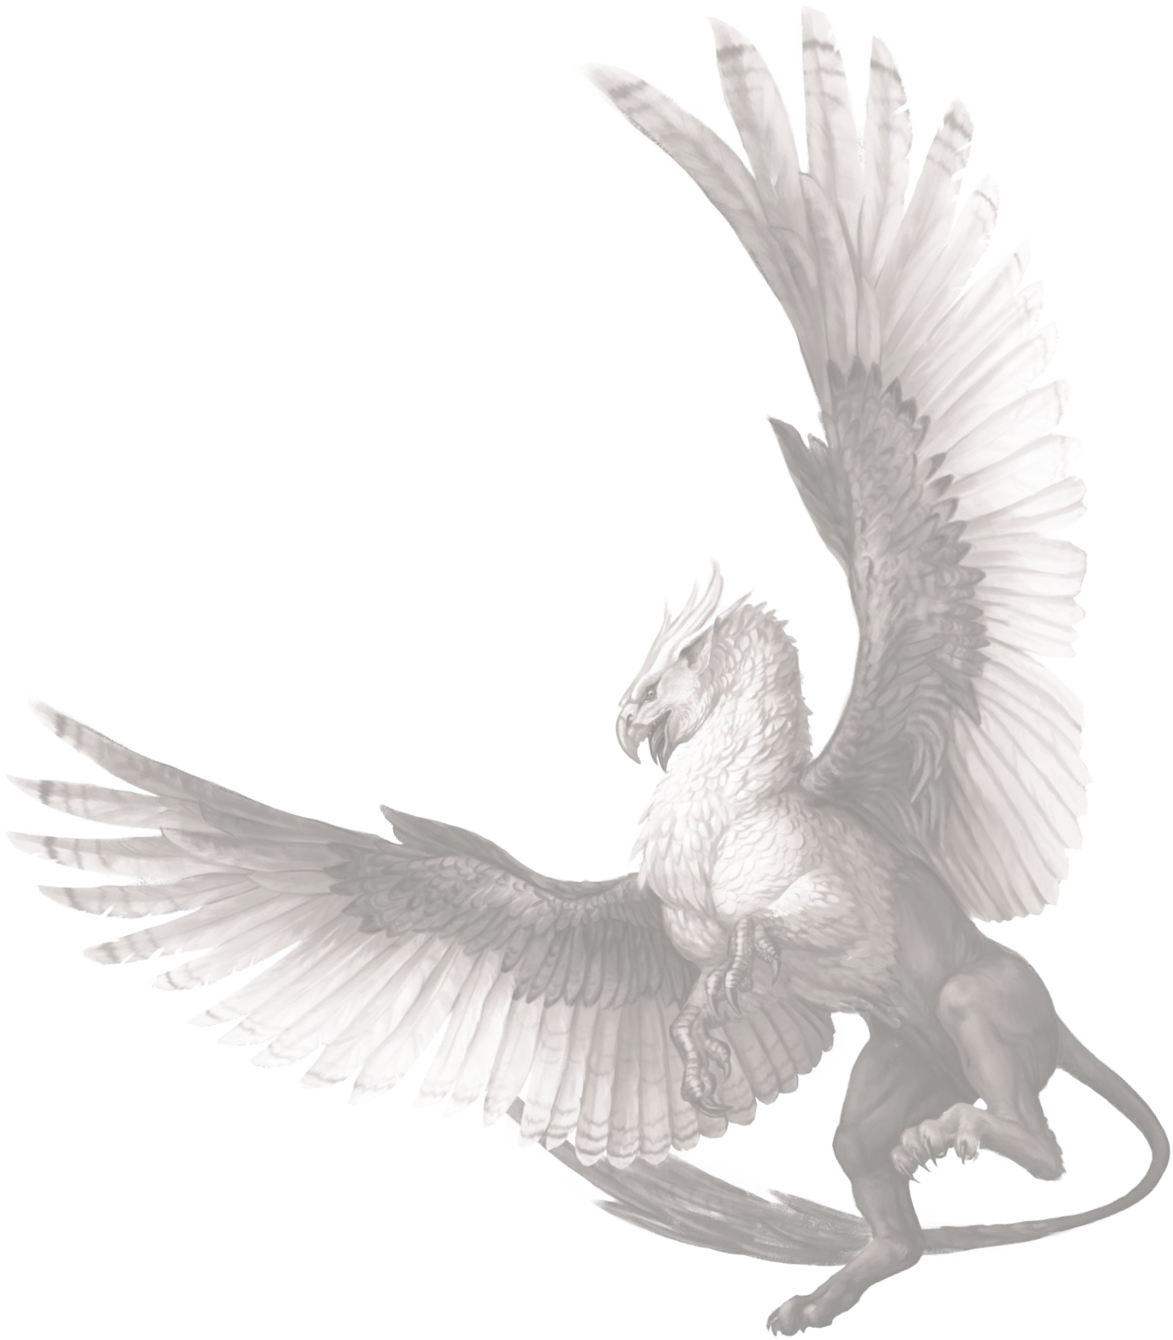
\includegraphics[width=\linewidth, keepaspectratio]{\art/griffin.png}
}

\end{multicols}

\begin{tikzpicture}[overlay]
  \node at (8.6, -5.3) {
    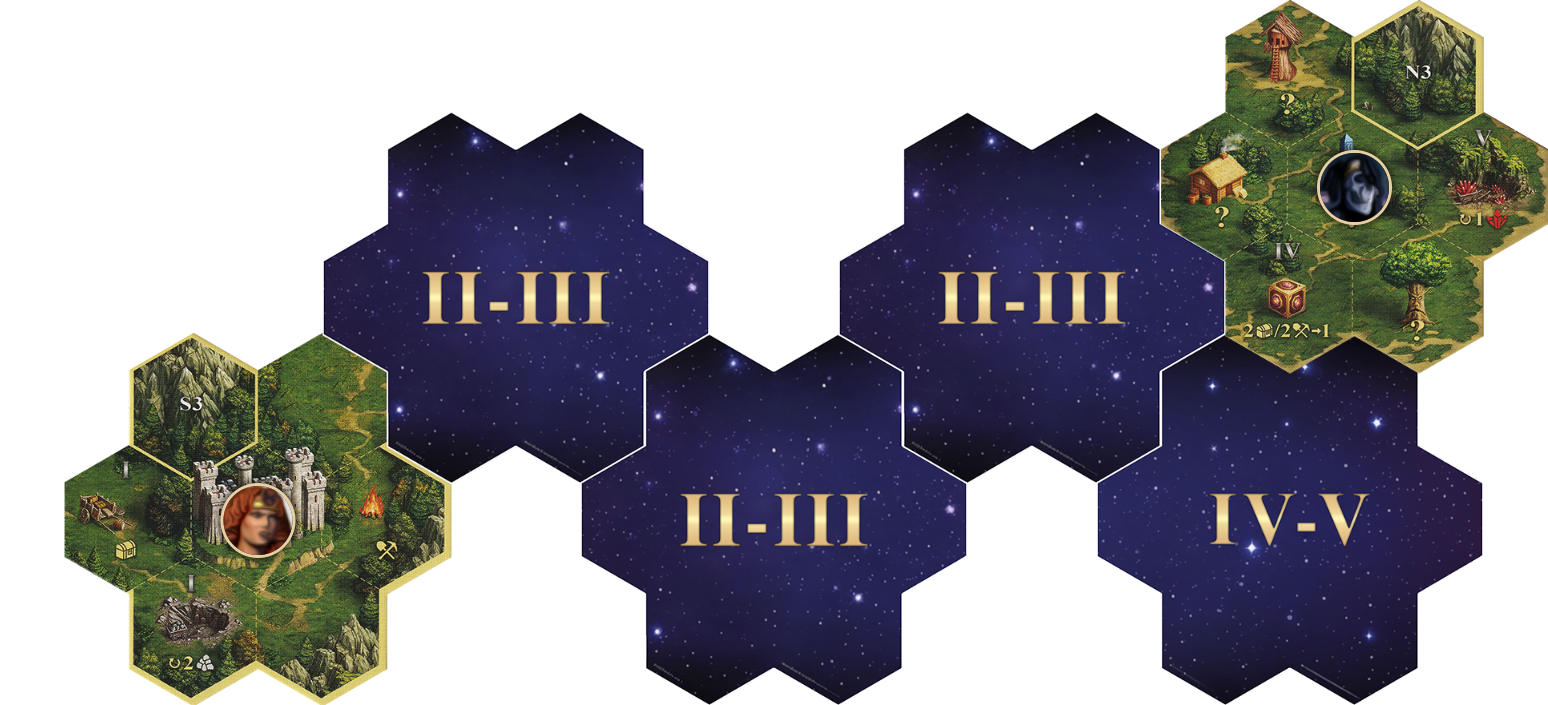
\includegraphics[width=\textwidth]{\_assets/maps/castle_greek_gift.png}
  };
  \node at (10, -2.0) {\large{{\textbf{\textcolor{darkcandyapplered}{F3}}}}};
\end{tikzpicture}

\newpage

\begin{multicols*}{2}

\subsection*{\MakeUppercase{The story}}

\textbf{Distant Threat}

Catherine Ironfist rubbed her tired, worn thumb across the image of her father, King Gryphonheart, in a locket.
She wanted to remember the good, valiant parts of his life rather than his actions in unlife.
Her gaze turned to her cracked skin and mangled thumbnail, and it reminded her of how hard she had fought to be where she was.

The weight of Erathia rested on her shoulders.
It had only been weeks since the siege and recapture of Steadwick, and resources, as well as manpower, were in short supply.
Still, with time, the stony seat of the castle would be sufficient to further liberate the realm.

One such problem was weighing on her mind.
After replacing the locket in her hand with a missive, she re-read a particular entry about a rising necromancer named Vhidhax.
Rumors were that the fiend had stolen precious artifacts that further enhanced his power over the dead.
While rumors are usually best left to fishwives and children, this one aligned with information about an army growing in strength, and she dreaded the thought of the two problems colliding and crashing over her weary crown.

Late that evening, Catherine was venting to Rion about the relative drudgery of rebuilding Steadwick.
She'd just about fallen asleep in her chair when a heavy knock turned her attention to the room's large door that sported intricately carved shields from various long-gone baronies.

The wooden portal flung open before she could spring up, revealing a wide-eyed and panicked guard.
No words came from the man; whatever haunted him seemed absolute.
Instead, he merely pointed with a trembling hand toward the window across the room.

Catherine shot a look at Rion before the two darted toward the open air of the rectangular window.
What they saw shocked them, too, and while Catherine's heart sank, she gripped Rion's shoulder with surprising strength.
When he looked back at her with a slight wince, she only returned a stony look of resolve.

Danger had come to Steadwick again.
Atop a hill in the far distance, overlooking many of the defenseless farmsteads Catherine had in her charge, a predator swept its gaze like a wolf might hungrily eye sheep.
A magnificently terrifying azure hue wafted from a Ghost Dragon's massive, extended wings like an ethereal heat haze.

\textbf{Reverent Allies}

While Catherine trusted her horse, having fought tooth and nail with the battle-hardened steed for as long as she could remember, it shuddered in hesitation as they approached the majestic, columned main building of the settlement.
Catherine had also felt the almost unsettling holy power in the area when, suddenly, the sound of rushing wings caught her attention.
Her gaze snapped upward to catch sight of something approaching.

The early morning sun was bright, and the figure that swooped low was in front of it.
The silhouette of wings was visible, and Catherine thought it to be a Gryphon at first.
However, as it closed in on them, it became apparent it was the shape of a man with wings instead.
It caught Catherine's horse off guard, and she had to catch the reins and wrench them hard to steady herself and calm the frightened animal before it could fling her from her seat.

With lightning speed, the figure landed mere feet from them to reveal the stubbled, handsome face of a young man with golden, curled locs and impressively robust bronze armor sculpted to his muscular form.
He was one of the famed Archangels to have stayed near Steadwick after Catherine's victory.
While the forces behind her fell to their knees in reverence, she only nodded with stern resolve.

With a deeper, and more reverberating voice than any man, the angel was first to speak.
``Queen Catherine.
I expected you might come when I spied the rot taking form in the hills.''

Catherine responded with a smile.
It was good to see she still had allies; her forces would need bolstering to take on the undead.
``It's good to see you, my friend,'' she said.
``It seems Steadwick is threatened again, and I ride to root out the evil before it can seed.
Would you join me at my side?''

``Of course, my queen!'' the angel barked.
``Combined, no evil can thwart our advance!'' As the final words left his lips and began to echo, he drew his weapon.
The longsword ignited as it left its sheath, and its blazing glory had most of those kneeling averting their eyes.
Immediately after, he took to the air and began circling the area again.
Catherine smiled wide as she watched more angels appear, then looked back to her forces and extended an open palmed arm forward in a command to march.

\textcolor{darkcandyapplered}{Add a Few Archangels to your army.}

\textbf{Bait And Switch}

Catherine couldn't wait to drive her sword through the heart of the Ghost Dragon, then lop the head from the one commanding it.
She pushed her powerful mount forward, charging toward the waiting, taunting foes.
While the great number of shambling undead, mostly animated citizens from nearby townships, was impossible to ignore, they wouldn't stop her.
With a thunderous crash, she slammed past the forward lines, knocking off limbs and cracking bones.

Seconds later, she was halfway through the mass of bodies when the stench of rotten flesh and the true immensity of her enemy's numbers hit her.
Dread Knights flanked the dragon she'd been racing towards.
Worse still, a robed, decrepit-looking figure was watching from the rear of the enemy lines.
Despite its wretched appearance, it had an immensely powerful presence to it.
A stinging tingle shot up Catherine's spine as she felt, more than saw, its eyes return her gaze.
More than she could take on alone, she swung her steed in a circle to reform with her mounted allies, then looked to the sky just as an Archangel came crashing down onto the dragon.

Shockingly, instead of slamming into the beast, the angel flew through it like it was made of air.
He hit the ground with a crunching thud before, suddenly, the dragon's image began to shift and shimmer, then disintegrate.
The Dread Knights did the same, and replacing them were throngs of further undead that now threatened to encircle Catherine and her forward forces.

Catherine's eyes shot toward what she believed was the necromancer.
It stood motionless a moment longer before cackling laughter cut through the air, and its image wafted away into the night air just as the others had.

It was a trap.
The necromancer and his strongest forces were not there, and Catherine would have to fight her way out from under a crush of undead, wasting precious time and lives.

\begin{itemize}
  \item \textcolor{darkcandyapplered}{Replace the Ghost Dragons and Dread Knights with \bronze\ neutral Zombies and Skeletons.}
  \item \textcolor{darkcandyapplered}{Play ``Cloak of the Undead King IV'' and ``Cloak of the Undead King VI'' onto the packs of Zombies and Skeletons, respectively.}
  \item \textcolor{darkcandyapplered}{Remove the AI Might and Magic Deck from the game, the undead fight on their own.}
\end{itemize}


\textbf{The Chase Begins}

Catherine huffed, sweat beading on her forehead as the last undead fell with wet thuds.
Her forces were strong, and simple reanimations weren't the kind of threat to stop them.
She just hoped… Her stomach churned as her gaze turned back to Steadwick.

An orange glow, far too bright for torchlight, was coming from the castle.
As she watched in horror, thick black smoke began to rise from the towers and parapets.
Steadwick was burning.

Rion quickly caught up to her, his horse panting as hard as he was.
He began to speak but couldn't find the words as his mind raced.
Instead, he placed a hand on his queen's shoulder.

The necromancer had played his opening move and won.

Just before Catherine turned to her regrouping forces, she spotted the spectral blue of the real Ghost Dragon in the distance.
Its work destroying Steadwick's defenses had been finished.

Archangels circled overhead, and Catherine threw her head to the sky, tears welling at the thought of losing what she had worked so hard to build.
``Find him!'' she roared, addressing whatever gods were listening as well as the angels above.

``Is that… wise?'' Rion asked softly.

Catherine responded with fire in her eyes.
``What good is rebuilding a ruin when the fiend will just continue to play his tricks?'' she said.
``No.
If we want to save Steadwick, we have to end him before he can further strengthen himself.''

\begin{itemize}
  \item \textcolor{darkcandyapplered}{Remove Archangels from your army.}
  \item \textcolor{darkcandyapplered}{Keep the rest of your forces and resources for the next Scenario.}
  \item \textcolor{darkcandyapplered}{Reset your Hero per the normal campaign rules.}
\end{itemize}

\columnbreak

\begin{center}
  \framedimage[0.8\linewidth]{\art/ghost_dragon.jpg}
\end{center}

\end{multicols*}
